\section{esercizio 13}
\textit{\textbf{Descrizione:} Scaricare la function cremat1 che crea sistemi lineari $m \times n$, con $m \geq n$, la cui soluzione (nel senso dei minimi quadrati) è il vettore $x = (1 \cdots n)^{T}$. Eseguire, quindi, lo script Matlab (vedere esercizio) per testare le function dei precedenti esercizi.}\newline
\noindent\emph{Soluzione: }\newline
una volta scaricata la function cremat1
\\~\\
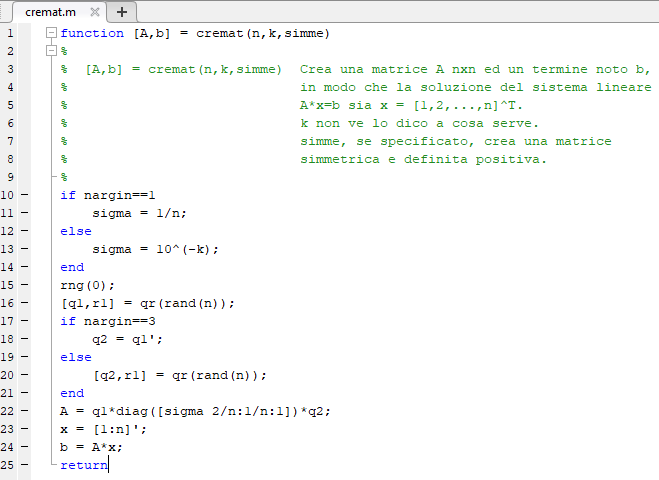
\includegraphics[width=1.3\linewidth]{img/cremat.png}\\~\\
ed aver eseguito lo script
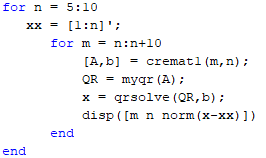
\includegraphics[width=.8\linewidth]{img/ex13.png}\\~\\
otteniamo i seguenti risultati
\\~\\
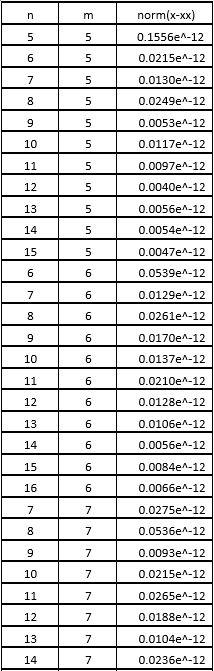
\includegraphics[width=.5\linewidth]{img/tabella13x1.png}\newpage
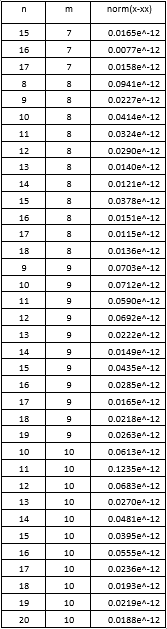
\includegraphics[width=.5\linewidth]{img/tabella13x2.png}